\documentclass[a4paper]{article}

%% Language and font encodings
\usepackage[english]{babel}
\usepackage[utf8x]{inputenc}
\usepackage[T1]{fontenc}
\usepackage{listings}
\usepackage{booktabs}

%% Sets page size and margins
\usepackage[a4paper,top=3cm,bottom=2cm,left=3cm,right=3cm,marginparwidth=1.75cm]{geometry}

%% Useful packages
\usepackage{amsmath}
\usepackage{graphicx}
\usepackage[colorinlistoftodos]{todonotes}
\usepackage[colorlinks=true, allcolors=blue]{hyperref}

\title{Creating TRELIS Mesh From MCNP Input}
\author{YeCheng}

\begin{document}
\maketitle



\section{Fixing The Installation Problems}
MCNP-Trelis-plugins used to cause some problems on different user's computer that the plugins were not recognized even though all the soft links created by
the installation script were successfully put in the correct place. There are two possible errors making the Trelis-plugins not being detected: \\ \\
1) \textbf{libMOAB.so.0} is not found because that the \textbf{LD\_LIBRARY\_PATH} has not been set in new user's \textbf{bashrc} file.\\
2) \textbf{libarmadillo.so.6} is not found because the package \textbf{libarmadillo-dev}, on which Trelis-plugins have a dependence, has not been
   installed on new user's computer.\\ \\
The detailed Trelis-fixing instruction , newly updated Trelis\_installation\_instruction and \textbf{install.sh} are in the \textbf{\textit{Installation}} folder in this
repository.



\section{Importing and Meshing}
\subsection{Import MCNP Scripts Using MCNP-Trelis-Plugins}
An MCNP script can be simply imported by Trelis using the following command,
\begin{lstlisting}
 import MCNP <MCNP_file_name>
\end{lstlisting}
and then the MCNP-Trelis-Plugins will automatically read the MCNP script and generate the geometry and materials according to that. For example, a KSU-single-fuel-model has been
used to test the importing and meshing. After importing it, Trelis generates a 3-D model as shown in Fig.1. 
\begin{figure}[th!]
\centering
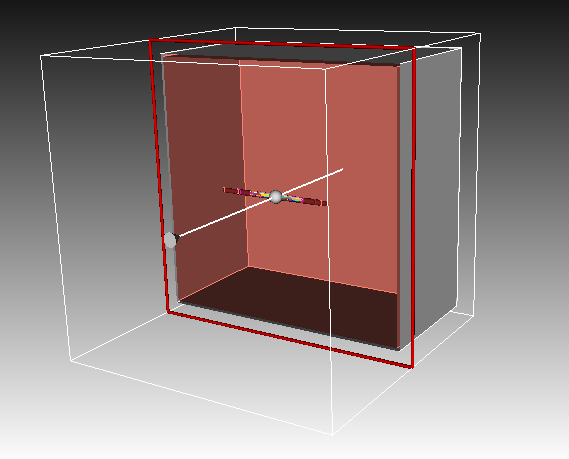
\includegraphics[width=.6\textwidth]{fig1}
\caption{3-D Model Generated by MCNP-Trelis-plugins}
\end{figure}
All the cells in MCNP are transfered into the volumes and the materials are assigned to the volumes respectively.
\subsection{Creating the Mesh}
The simplest way of generating the mesh for all the volumes in the model is to use the following syntax
\begin{lstlisting}
 mesh volume all
\end{lstlisting}
and Trelis will automatically mesh the all the volumes such as the coolant, cladding, fuel region and Zr rod etc. The shortcoming 
of this method is that some volumes like the fuel rod may need finer meshing and pie slicing and the auto-scheme meshing be too coarse. Fig.2 shows the auto-generated mesh
for the example model.
\begin{figure}[th!]
\centering
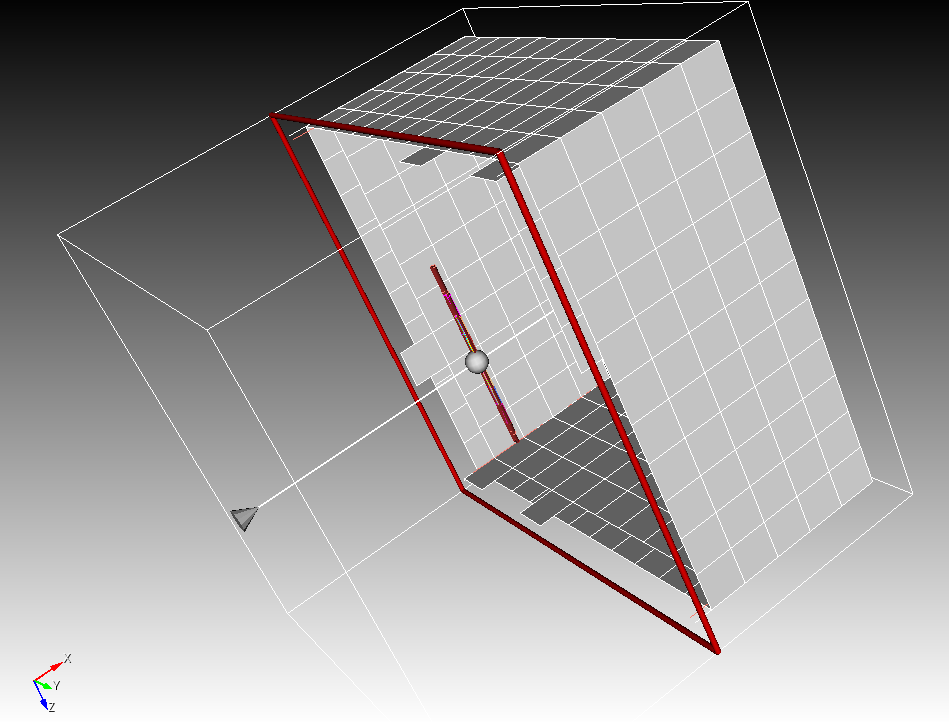
\includegraphics[width=.6\textwidth]{fig2}
\caption{Auto-scheme Trelis Meshing}
\end{figure}\\
An alternative way, and a more implicit way, is to mesh the volumes by user's definition. User can select the meshing scheme and how fine the mesh should be for each volume by using
\begin{lstlisting}
 <volume> Scheme <Scheme-selection>
\end{lstlisting}
and
\begin{lstlisting}
 remesh volume <volume #> <volume size>.
\end{lstlisting}























\end{document}